\documentclass[conference,a4paper]{IEEEtran}
\IEEEoverridecommandlockouts
\usepackage[utf8]{inputenc}
\usepackage[T1]{fontenc}
\usepackage{cite}
\usepackage{amsmath,amssymb}
\usepackage{graphicx}
\usepackage[table]{xcolor}
\usepackage{booktabs}
\usepackage{tabularx}
\usepackage[hyphens]{url}
\def\UrlFont{\rmfamily}
\definecolor{TableHeader}{gray}{0.88}
\definecolor{TableGroup}{gray}{0.95}
\definecolor{PanelRule}{gray}{0.6}
% Generated by scripts/make_tables.py from evidence/verified_numbers.json. Do not edit by hand.
\newcommand{\nExact}{38{,}382}
\newcommand{\nSevere}{363}
\newcommand{\nOutcomes}{38{,}745}
\newcommand{\nStations}{171}
\newcommand{\nCities}{97}
\newcommand{\nDates}{332}
\newcommand{\nHist}{31{,}622}
\newcommand{\nHistSevere}{306}
\newcommand{\devStationDays}{91{,}080}
\newcommand{\devValid}{55{,}192}
\newcommand{\devRejected}{35{,}888}
\newcommand{\devStations}{178}
\newcommand{\devCities}{99}
\newcommand{\devRejectedShare}{39}
\newcommand{\maeClim}{52.82}
\newcommand{\maeCal}{46.74}
\newcommand{\maeWx}{43.86}
\newcommand{\maePers}{27.47}
\newcommand{\maeHist}{28.09}
\newcommand{\rmsePers}{48.13}
\newcommand{\rmseHist}{46.20}
\newcommand{\dWxClim}{$-$8.96}
\newcommand{\dWxClimAbs}{8.96}
\newcommand{\dWxClimLo}{$-$12.49}
\newcommand{\dWxClimHi}{$-$5.61}
\newcommand{\dWxClimLoAbs}{12.49}
\newcommand{\dWxClimHiAbs}{5.61}
\newcommand{\dWxClimRel}{17.0}
\newcommand{\dWxCal}{$-$2.88}
\newcommand{\dWxCalAbs}{2.88}
\newcommand{\dWxCalLo}{$-$4.47}
\newcommand{\dWxCalHi}{$-$1.54}
\newcommand{\dWxCalLoAbs}{4.47}
\newcommand{\dWxCalHiAbs}{1.54}
\newcommand{\dWxCalRel}{6.2}
\newcommand{\dHistPers}{0.61}
\newcommand{\dHistPersAbs}{0.61}
\newcommand{\dHistPersLo}{$-$0.41}
\newcommand{\dHistPersHi}{1.70}
\newcommand{\dHistPersLoAbs}{0.41}
\newcommand{\dHistPersHiAbs}{1.70}
\newcommand{\dHistPersRel}{2.2}
\newcommand{\dHistWx}{$-$16.39}
\newcommand{\dHistWxAbs}{16.39}
\newcommand{\dHistWxLo}{$-$19.71}
\newcommand{\dHistWxHi}{$-$13.43}
\newcommand{\dHistWxLoAbs}{19.71}
\newcommand{\dHistWxHiAbs}{13.43}
\newcommand{\dHistWxRel}{36.8}
\newcommand{\pHistPers}{0.075}
\newcommand{\foldMaeMin}{22.96}
\newcommand{\foldMaeMax}{71.47}
\newcommand{\nFoldsClimBetter}{2}
\newcommand{\nFoldsPersBetter}{4}
\newcommand{\slidingWx}{59.92}
\newcommand{\slidingClim}{59.35}
\newcommand{\nSpatial}{26{,}228}
\newcommand{\nSpatialHigh}{3{,}911}
\newcommand{\spatialStations}{176}
\newcommand{\spatialDates}{222}
\newcommand{\maeSpatialRef}{47.34}
\newcommand{\spStation}{0.20}
\newcommand{\spStationLo}{0.17}
\newcommand{\spStationHi}{0.24}
\newcommand{\spStationRel}{0.4}
\newcommand{\spStationHigh}{0.70}
\newcommand{\spStationHighLo}{0.55}
\newcommand{\spStationHighHi}{0.82}
\newcommand{\spCity}{0.30}
\newcommand{\spCityLo}{0.22}
\newcommand{\spCityHi}{0.37}
\newcommand{\spCityRel}{0.6}
\newcommand{\spCityHigh}{0.93}
\newcommand{\spCityHighLo}{0.68}
\newcommand{\spCityHighHi}{1.13}
\newcommand{\spCluster}{1.94}
\newcommand{\spClusterLo}{1.58}
\newcommand{\spClusterHi}{2.34}
\newcommand{\spClusterRel}{4.1}
\newcommand{\spClusterHigh}{6.85}
\newcommand{\spClusterHighLo}{5.51}
\newcommand{\spClusterHighHi}{7.94}
\newcommand{\spRegion}{2.18}
\newcommand{\spRegionLo}{1.52}
\newcommand{\spRegionHi}{2.93}
\newcommand{\spRegionRel}{4.6}
\newcommand{\spRegionHigh}{9.97}
\newcommand{\spRegionHighLo}{3.68}
\newcommand{\spRegionHighHi}{14.69}
\newcommand{\spEast}{3.29}
\newcommand{\spNorth}{2.60}
\newcommand{\biasWxGood}{$+$26.1}
\newcommand{\biasWxPoor}{$-$124.4}
\newcommand{\biasWxVeryPoor}{$-$205.9}
\newcommand{\biasPersVeryPoor}{$-$51.8}
\newcommand{\biasHistVeryPoor}{$-$110.0}
\newcommand{\nPoorPlus}{4{,}713}
\newcommand{\nVeryPoorPlus}{2{,}406}
\newcommand{\poorPlusShare}{12}
\newcommand{\sevMaxWx}{201.6}
\newcommand{\sevShortWx}{258.6}
\newcommand{\sevPersReach}{147}
\newcommand{\sevHistReach}{1}
\newcommand{\sevShortPers}{50.8}
\newcommand{\sevShortHist}{125.1}
\newcommand{\sevStations}{40}
\newcommand{\sevCities}{29}
\newcommand{\sevFolds}{11}
\newcommand{\covEighty}{78.2}
\newcommand{\covNinety}{87.6}
\newcommand{\covNinetyLo}{84.9}
\newcommand{\covNinetyHi}{89.7}
\newcommand{\covEightyLo}{75.4}
\newcommand{\covEightyHi}{80.7}
\newcommand{\covFoldMin}{69.0}
\newcommand{\covFoldMax}{95.5}
\newcommand{\covSplitGood}{92.0}
\newcommand{\covSplitSat}{98.7}
\newcommand{\covSplitMod}{91.4}
\newcommand{\covSplitPoor}{54.0}
\newcommand{\covSplitVeryPoor}{8.7}
\newcommand{\covMondVeryPoor}{14.7}
\newcommand{\covCqrVeryPoor}{17.6}
\newcommand{\covCqrGood}{76.3}
\newcommand{\covSplitPoorPlus}{32.7}
\newcommand{\covSplitLow}{96.4}
\newcommand{\shiftCorr}{-0.92}
\newcommand{\covPostMonsoon}{73.8}
\newcommand{\underPzero}{27.1}
\newcommand{\overPzero}{24.7}
\newcommand{\underPtwo}{14.2}
\newcommand{\overPtwo}{41.7}
\newcommand{\dUnder}{12.9}
\newcommand{\dUnderLo}{10.0}
\newcommand{\dUnderHi}{15.9}
\newcommand{\dOver}{17.0}
\newcommand{\dOverLo}{14.0}
\newcommand{\dOverHi}{20.0}
\newcommand{\topUnder}{4.6}
\newcommand{\topOver}{85.3}
\newcommand{\topHighUnder}{37.5}
\newcommand{\highUnderPtwo}{86.3}
\newcommand{\pThreeTenFolds}{11}
\newcommand{\pThreeTenMet}{7}
\newcommand{\pThreeTenUnder}{11.1}
\newcommand{\pThreeTenOver}{48.7}
\newcommand{\pThreeTenInfeasible}{1}
\newcommand{\pThreeFiveFolds}{10}
\newcommand{\pThreeFiveMet}{6}
\newcommand{\pThreeFiveUnder}{6.2}
\newcommand{\pThreeFiveOver}{68.1}
\newcommand{\pThreeFiveInfeasible}{2}
\newcommand{\camsVerified}{6}
\newcommand{\camsPlanned}{36}
\newcommand{\camsDates}{42}
\newcommand{\camsFailed}{1}
\newcommand{\checksCompared}{144}

\newcommand{\pmtwo}{PM$_{2.5}$}
\newcommand{\pmten}{PM$_{10}$}
\newcommand{\ozone}{O$_3$}

\begin{document}

\title{AirGuard India: What Mean Error Conceals in Availability-Aware Next-Day Air Quality Forecasts}

\author{\IEEEauthorblockN{Nishanth R}
\IEEEauthorblockA{\textit{Department of Artificial Intelligence and Data Science}\\
\textit{Rajalakshmi Engineering College}\\
Chennai, Tamil Nadu, India\\
nishanth.r.2024.aids@rajalakshmi.edu.in}}

\maketitle

\begin{abstract}
Next-day air quality index (AQI) forecasts are usually judged by mean error, yet the decisions they inform depend on which days and places the errors fall. We ask whether an acceptable average conceals failures in geographic transfer, severe pollution, prediction intervals and warnings. Using Central Pollution Control Board (CPCB) measurements distributed by OpenAQ, we evaluate forecasts of a three-pollutant CPCB-style AQI reconstructed from PM2.5, PM10 and ozone, issued at 20:00 Indian Standard Time for the following day under a rule that admits only information available before issue. Twelve expanding chronological folds supply \nExact{} exact station-day targets and \nSevere{} Severe outcomes known only as lower bounds, from \nStations{} stations in \nCities{} cities. A Ridge model driven by forecast weather lowers mean absolute error from \maeClim{} to \maeWx{} AQI units against climatology, with a paired 95 percent interval for the reduction of \dWxClimHiAbs{} to \dWxClimLoAbs{}, but adding measurement history does not establish an advantage over persistence. Withholding whole regions raises error by \spRegion{} units overall and by \spRegionHigh{} units on Poor-or-worse days. Nominal 90 percent conformal intervals cover \covNinety{} percent of exact outcomes but \covSplitVeryPoor{} percent of Very Poor ones, and no interval reaches the Severe lower bound. Warning from an upper quantile cuts under-warning from \underPzero{} to \underPtwo{} percent while raising over-warning from \overPzero{} to \overPtwo{} percent. The operational atmospheric-composition correction is incomplete and the final 90-day test remains sealed.
\end{abstract}

\begin{IEEEkeywords}
air quality forecasting, forecast availability, geographic generalization, conformal prediction, severe pollution episodes, warning decisions
\end{IEEEkeywords}

\section{Introduction}
A forecast issued this evening for tomorrow's air quality is useful only if it could have been produced this evening. India's daily air quality index (AQI) maps pollutant concentrations to six categories, from Good to Severe, that underlie public advisories~\cite{cpcb2014}. A retrospective experiment can silently borrow observations or model runs that arrived after issue, a recurring source of irreproducible machine-learning results~\cite{kapoor2023}, so input timing is part of the forecast.

Mean error summarizes a forecast over the days that happen to be frequent, and it hides four properties that matter in use. A model can reproduce familiar monitors yet fail where none contributed to training~\cite{pant2019}, and the days that drive warnings are too rare to move the average. A prediction interval can meet its nominal coverage overall while missing most polluted days, because distribution-free guarantees are marginal, not conditional~\cite{foygelbarber2021}. And a warning has two different errors, a missed category and an unnecessary alert, whose balance no single accuracy score expresses~\cite{murphy1977}.

Prior work treats these properties separately. Operational systems for Delhi underpredict Severe episodes~\cite{jena2021,govardhan2024}, post-processing of Copernicus Atmosphere Monitoring Service (CAMS) forecasts is established at European stations~\cite{petetin2022,bertrand2023,riccio2024}, and a single-station Indian study with conformal intervals reports lower skill in polluted regimes~\cite{lawrence2026}. It remains unresolved whether one multi-city Indian experiment under a single availability contract supports consistent claims across all four, with open-ended Severe outcomes treated as bounds.

AirGuard India fixes the issue time at 20:00 Indian Standard Time (IST) for the next calendar day and asks four research questions.
\textbf{RQ1}: What do availability-safe forecast weather and recent measurement history contribute beyond climatology and persistence?
\textbf{RQ2}: How does error change when stations, cities, urban clusters and regions are withheld from training?
\textbf{RQ3}: Can acceptable marginal interval coverage hide failure in high-pollution conditions?
\textbf{RQ4}: How do conservative warning rules trade missed severity categories against excess alerts?

The contributions are empirical: (1)~a traceable target and availability contract, with Severe outcomes kept as lower bounds and inputs admitted only with evidence that they precede issue; (2)~a paired evaluation over 12 chronological folds and 36 geographic exclusions; and (3)~a reliability audit that conditions interval coverage and warning losses on observed severity and separates completed evidence from an unfinished CAMS correction and from the live application (Fig.~\ref{fig:architecture}).

\section{Related Work}
\subsection{Operational Forecast Calibration}
For CAMS post-processing, the correction that minimizes continuous ozone error is not the one that best detects exceedances~\cite{petetin2022}, a model pooled over European stations rivals station-specific ones~\cite{bertrand2023}, and static calibration does not uniformly beat persistence~\cite{casciaro2022}. AirGuard's completed results use no CAMS field.

\subsection{Indian Forecasting and Geographic Generalization}
Operational Delhi systems are scored by category and miss events above AQI 400~\cite{jena2021,govardhan2024}. Evaluation design changes conclusions: cross-validation that ignores temporal or spatial dependence overstates skill~\cite{roberts2017}. Withholding whole locations exposes this optimism in pollution mapping~\cite{just2020}.

\subsection{Uncertainty and Warning Decisions}
Split conformal prediction gives intervals with marginal coverage under exchangeability~\cite{lei2018}, and conformalized quantile regression (CQR) adapts their width~\cite{romano2019}. Dependence and drift weaken the guarantee~\cite{barber2023}, and exact conditional coverage is unattainable without assumptions~\cite{foygelbarber2021}. Evaluation restricted to observed extremes can reward overforecasting~\cite{lerch2017}, and warning value depends on the user's cost--loss ratio~\cite{murphy1977}, so excess alerts are a cost.

\textit{Positioning.} No estimator here is new. Rather than introducing one, AirGuard contributes an availability-constrained evaluation framework that links temporal skill, geographic transfer under station, city, urban-cluster and regional holdouts, open-ended Severe outcomes treated as lower bounds, severity-conditioned uncertainty and two-sided warning losses on the same Indian station-day population, while keeping completed evidence separate from an unfinished CAMS correction and from the live deployment. None of the studies cited above reports these properties jointly.

\begin{figure*}[!t]
\centering
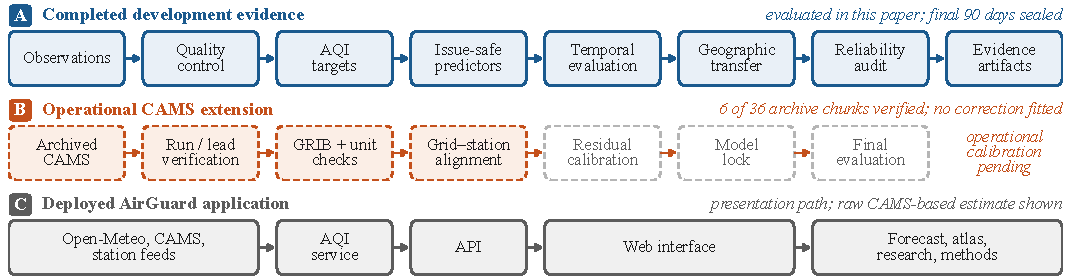
\includegraphics[width=\textwidth]{figures/fig1_architecture.pdf}
\caption{Evidence boundaries. Lane A: completed development evidence evaluated here. Lane B: operational CAMS extension; tinted dashed stages are partially complete and grey dashed stages have not started. Lane C: deployed application, a separate presentation path.}
\label{fig:architecture}
\end{figure*}

\section{Data and Target Construction}
\subsection{Station Cohort and Quality Control}
The Central Pollution Control Board (CPCB) is the measuring authority; OpenAQ redistributes its hourly records and is not the source of the index values built here~\cite{openaq2026}. From 481 CPCB locations in 255 cities that were active on or after 1 September 2026 and report \pmtwo{}, \pmten{} and ozone (\ozone{}) in mass units, a rule stratified by city size selected 181, and 180 were acquired for 19 February 2025 to 7 October 2026. This conditions on surviving monitors. An hourly bin must span one hour with at least 75\% coverage, no provider flag, and a finite positive value. Exact zeros and runs of six or more identical values are rejected; statistical spikes and \pmtwo{} above \pmten{} are flagged but kept. Before the sealed interval, \devValid{} of \devStationDays{} station-days (\devStations{} stations, \devCities{} cities) have a valid target; the rest stay in a rejection ledger.

\subsection{Three-Pollutant AQI and Severe Censoring}
The target is a three-pollutant CPCB-style AQI, not the officially issued index. Each pollutant needs 16 distinct hours in the target day. Particulate matter uses the 24-hour mean; \ozone{} uses the largest complete trailing eight-hour mean, or the one-hour bands of~\cite{cpcb2014} above 208~$\mu$g\,m$^{-3}$. For concentration $C$ between breakpoints $(C_L, C_H)$ with index limits $(I_L, I_H)$,
\begin{equation}
I_p(C) = I_L + \frac{I_H - I_L}{C_H - C_L}\,(C - C_L), \quad y_{s,d} = \max_{p} I_p(C_{p,s,d}),
\label{eq:aqi}
\end{equation}
for pollutant $p$, station $s$ and day $d$. Every valid target is supported by \pmtwo{}, \pmten{} and \ozone{} only, so the index can fall below the official one when an unmeasured gas dominates. Above the last closed breakpoint the CPCB scale is open-ended, and the target is recorded as $y_{s,d} \ge 401$, a lower bound and not a value. Such days are excluded from training and from exact error and coverage denominators but kept for category, shortfall and warning diagnostics.

\section{Availability Contract and Models}
\subsection{Issue-Time Contract}
The target is the IST calendar day $D$, issued at 20:00 on $D-1$ (Fig.~\ref{fig:timeline}a). Weather comes from the Open-Meteo archive of earlier Global Forecast System (GFS) runs, taking for each target hour the value from a run initialized at least 48 hours before, so every value was forecast, not observed~\cite{openmeteo2026}. Measured history is limited to hourly bins ending by 17:00. OpenAQ records no ingestion time, so this three-hour latency is an assumption on which all history-based results are conditional. Fire detections and short-lead CAMS fields are excluded because their publication times could not be established.

\subsection{Forecast Models}
Climatology is the station's training-window mean for the target month. Persistence is the AQI of the 24 hours ending at the cutoff. Three Ridge regressions share training-only median imputation and standardization, minimize squared error on exact training targets with an $\ell_2$ penalty fixed in advance at $\lambda = 10$, and clip predictions at zero. \textit{Calendar Ridge} uses six calendar terms and two coordinates. \textit{Weather Ridge} adds eleven daily summaries of forecast temperature, humidity, wind, precipitation, pressure, radiation and cloud. \textit{History Ridge} adds the persistence value and the six-hour \pmtwo{} mean and slope. History models are trained and scored only where history exists, and Weather Ridge is refitted on those rows, so a feature change is never confounded with a population change.

The protocol's primary comparison, a learned correction of operational CAMS global forecasts~\cite{cams2026}, is incomplete (Fig.~\ref{fig:architecture}, lane B). Of \camsPlanned{} archive chunks, \camsVerified{} have been retrieved, decoded and re-hashed for this paper. They yield \camsDates{} aligned forecast dates, too few for any fold, so no correction has been fitted; reanalysis is never substituted for archived forecasts.

\begin{figure*}[!t]
\centering
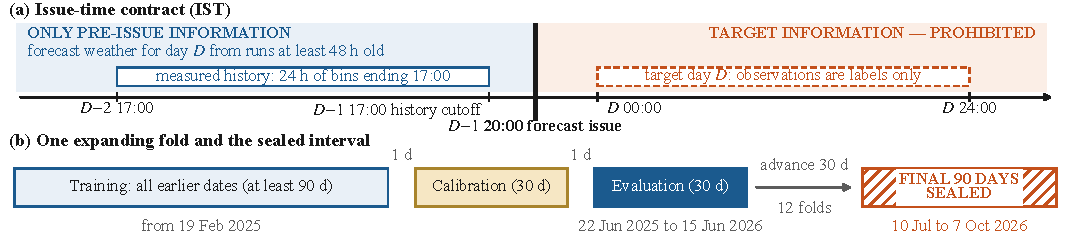
\includegraphics[width=\textwidth]{figures/fig2_timeline.pdf}
\caption{Leakage safeguards. (a)~Only information available before the 20:00 IST issue is admitted; target-day observations serve as labels only. (b)~One expanding fold with one-day embargoes; folds advance by 30 days and the final 90 days stay sealed.}
\label{fig:timeline}
\end{figure*}

\section{Evaluation Design}
\subsection{Temporal and Geographic Separation}
Whole dates move together. Each of 12 expanding folds trains on all earlier dates (at least 90), calibrates on the next 30 and evaluates on the following 30, with one-day embargoes and a 30-day advance (Fig.~\ref{fig:timeline}b); a station needs 30 valid training targets. Evaluation spans 22 June 2025 to 15 June 2026: \nStations{} stations, \nCities{} cities, \nDates{} dates, \nExact{} exact pairs and \nSevere{} censored Severe outcomes, with history for \nHist{} exact pairs. The last 90 dates, 10 July to 7 October 2026, are a sealed final test. Its rows are filtered out before any table is materialized, and scoring them requires a committed model-selection lock.

Spatial models train through 31 October 2025 and are evaluated from 2 November 2025 to 9 July 2026, which contains the winter. Stations, cities and urban clusters (single linkage at 25~km) are each assigned to ten groups from catalog metadata, and six regions are withheld in turn, giving 36 exclusions. Each excluded Weather Ridge is compared with an all-station reference on the same \nSpatial{} exact rows.

\subsection{Intervals and Warning Rules}
With sorted absolute calibration residuals $e_{(1)} \le \dots \le e_{(n)}$ of exact targets, the split interval at level $1-\alpha$ is
\begin{equation}
\mathcal{C}(x) = \bigl[\max(0, \hat{y} - q),\, \hat{y} + q\bigr], \quad q = e_{(\lceil (n+1)(1-\alpha) \rceil)},
\label{eq:split}
\end{equation}
at 80\% and 90\%. A Mondrian variant computes $q$ within each forecast category holding 30 calibration pairs. CQR uses gradient-boosted quantile trees at the 0.05 and 0.95 levels.

With observed category $c_i$ and issued category $w_i$ in $\{0,\dots,5\}$, under-warning is $w_i < c_i$ and over-warning is $w_i > c_i$. P0 issues the category of the Weather Ridge forecast; P1 and P2 issue those of the 0.5 and 0.75 quantile-tree forecasts after a one-sided conformal shift. P3 picks the smallest level $\tau$ whose finite-sample-corrected calibration-month under-warning rate is at most 10\% or 5\%~\cite{angelopoulos2024}, and abstains otherwise.

\subsection{Inference and Reproduction}
Mean absolute error (MAE) on exact targets is primary; root-mean-square error (RMSE) and bias are secondary. Paired differences use 5{,}000 moving seven-day calendar-block resamples~\cite{kunsch1989} that keep all stations of a date together. A Diebold--Mariano test on daily mean loss differences~\cite{diebold1995}, Holm-adjusted over four contrasts, is a date-weighted check. Refitting the frozen configuration on development dates reproduced all \checksCompared{} compared fold summaries exactly and supplied the row-level outputs used below; code, hashes and evidence files are in the repository.\footnote{\raggedright\url{https://github.com/nishaids/airguard-india}, branch \texttt{research/station-calibration}; run \texttt{287c87db04a6}; dataset \texttt{4761a5da60dd}.}

\begin{table}[!t]
\caption{Point Forecast Errors on Exact Development Targets}
\label{tab:point}
\centering
\footnotesize
\setlength{\aboverulesep}{0pt}\setlength{\belowrulesep}{0pt}\renewcommand{\arraystretch}{1.14}\setlength{\tabcolsep}{6pt}
\begin{tabularx}{\columnwidth}{X r r r}
\toprule
\rowcolor{TableHeader}\textbf{Model} & \textbf{MAE} & \textbf{RMSE} & \textbf{Bias}\\
\midrule
\rowcolor{TableGroup}\multicolumn{4}{l}{\textit{All exact pairs}: $n=38{,}382$, 171 stations, 332 dates}\\
Climatology & 52.82 & 74.42 & $-$8.21\\
Calendar Ridge & 46.74 & 69.49 & $-$19.18\\
Weather Ridge & 43.86 & 67.33 & $-$16.69\\
\midrule
\rowcolor{TableGroup}\multicolumn{4}{l}{\textit{History-available pairs}: $n=31{,}622$, 171 stations, 320 dates}\\
Weather Ridge, refitted on these rows & 44.47 & 68.24 & $-$17.67\\
Persistence & 27.47 & 48.13 & $+$0.97\\
History Ridge & 28.09 & 46.20 & $-$7.17\\
\bottomrule
\end{tabularx}
\\[3pt]
\parbox{\columnwidth}{\footnotesize AQI units. Bias: forecast minus observed. The two groups are different populations; censored Severe outcomes are excluded.}
\end{table}


\section{Results and Discussion}
\subsection{RQ1: Weather, History and Persistence}
Weather Ridge lowers MAE by \dWxClimAbs{} units (\dWxClimRel\%) relative to climatology (Table~\ref{tab:point}), with a 95\% interval of \dWxClimLo{} to \dWxClimHi{} (Fig.~\ref{fig:rq1}); forecast weather contributes \dWxCalAbs{} of this beyond calendar and coordinates (\dWxCalLo{} to \dWxCalHi{}). The gain is not uniform: climatology is better in \nFoldsClimBetter{} folds and with a 90-day sliding training window the pooled advantage disappears (\slidingWx{} against \slidingClim{}).

Recent history matters more than weather: where it exists it lowers Ridge MAE by \dHistWxAbs{} units (\dHistWxLo{} to \dHistWxHi{}). Yet History Ridge is not better than persistence. The difference is $+$\dHistPers{} (\dHistPersLo{} to $+$\dHistPersHi{}), persistence wins in \nFoldsPersBetter{} folds, including the three most polluted, and the date-weighted test does not reject equal accuracy (adjusted $p = \pHistPers$). All four conclusions hold for block lengths of 3 to 28 days.

\begin{figure}[!t]
\centering
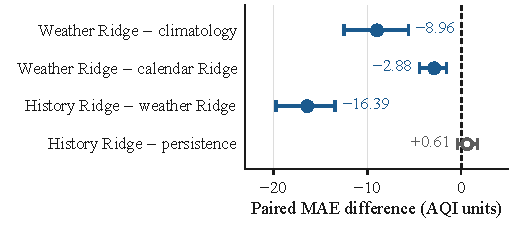
\includegraphics[width=\columnwidth]{figures/fig3_rq1.pdf}
\caption{RQ1. Paired station-day MAE differences with 95\% block-bootstrap intervals. Filled markers: interval excludes zero. Open marker: no established difference. The upper two contrasts use \nExact{} exact pairs, the lower two the \nHist{} pairs with history.}
\label{fig:rq1}
\end{figure}

\subsection{RQ2: Geographic Transfer}
Excluding locations from training raises error at every scale (Fig.~\ref{fig:transfer}a). The increase over the \maeSpatialRef-unit reference is \spStation{} (\spStationLo{} to \spStationHi{}) for stations, \spCity{} (\spCityLo{} to \spCityHi{}) for cities, \spCluster{} (\spClusterLo{} to \spClusterHi{}) for urban clusters and \spRegion{} (\spRegionLo{} to \spRegionHi{}) for regions, or \spStationRel\% to \spRegionRel\%. On the \nSpatialHigh{} Poor-or-worse pairs the same exclusions cost \spStationHigh{}, \spCityHigh{}, \spClusterHigh{} (\spClusterHighLo{} to \spClusterHighHi{}) and \spRegionHigh{} (\spRegionHighLo{} to \spRegionHighHi{}) units, concentrated in the North and East. A model without local history thus transfers to an unseen station in a seen city at almost no cost, but loses skill on polluted days when a whole airshed is new.

\subsection{RQ3: Severe Days and Interval Coverage}
\label{sec:rq3}
By observed category the Weather Ridge bias moves from \biasWxGood{} for Good to \biasWxPoor{} for Poor and \biasWxVeryPoor{} for Very Poor, against \biasPersVeryPoor{} for persistence where history exists. Weather Ridge issues a lower category than observed for all \nPoorPlus{} Poor-or-worse outcomes and forecasts none of the \nVeryPoorPlus{} Very Poor or Severe outcomes as Very Poor. On the \nSevere{} censored Severe days (\sevStations{} stations) its largest forecast is \sevMaxWx{}, a mean shortfall of at least \sevShortWx{} units. Recent measurements change this only in part (Fig.~\ref{fig:transfer}b): on the \nHistSevere{} Severe days with history, persistence reaches the lower bound on \sevPersReach{} and History Ridge on \sevHistReach{}.

\begin{figure*}[!t]
\centering
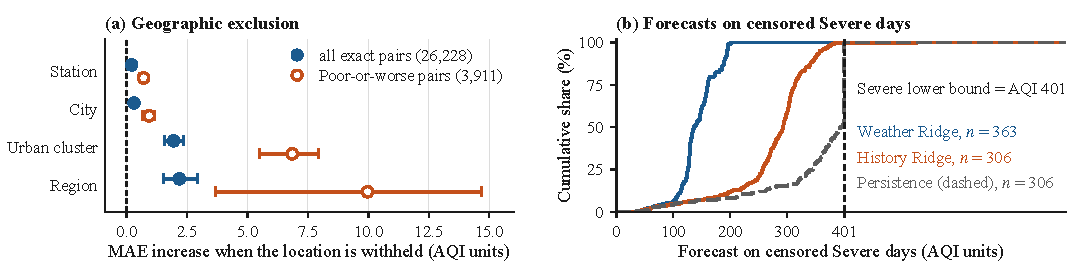
\includegraphics[width=\textwidth]{figures/fig4_transfer_severe.pdf}
\caption{RQ2 and RQ3. (a)~Increase in Weather Ridge MAE when a location is withheld from training (95\% block-bootstrap intervals): broader exclusion costs most on polluted days. (b)~Forecasts on the \nSevere{} censored Severe days; curves left of the bound are tail underprediction.}
\label{fig:transfer}
\end{figure*}

\begin{table}[!t]
\caption{Interval Coverage (\%) of Exact Targets, Overall and by Observed Category}
\label{tab:intervals}
\centering
\footnotesize
\setlength{\aboverulesep}{0pt}\setlength{\belowrulesep}{0pt}\renewcommand{\arraystretch}{1.14}\setlength{\tabcolsep}{2.5pt}
\begin{tabularx}{\columnwidth}{X c r r r r r r r}
\toprule
\rowcolor{TableHeader}\textbf{Method} & \textbf{Level} & \textbf{Overall} & \textbf{Good} & \textbf{Sat.} & \textbf{Mod.} & \textbf{Poor} & \textbf{V.~Poor} & \textbf{Width}\\
\midrule
Split & 80 & 78.2 & 77.7 & 93.9 & 84.2 & 20.2 & \textbf{0.0} & 124\\
Split & 90 & 87.6 & 92.0 & 98.7 & 91.4 & 54.0 & \textbf{8.7} & 169\\
Mondrian & 90 & 87.0 & 91.1 & 98.2 & 89.7 & 55.1 & \textbf{14.7} & 166\\
CQR & 90 & 87.1 & 76.3 & 99.4 & 96.1 & 60.4 & \textbf{17.6} & 162\\
\midrule
\rowcolor{TableGroup}Pairs & & 38{,}382 & 7{,}541 & 14{,}229 & 12{,}262 & 2{,}307 & 2{,}043 & \\
\bottomrule
\end{tabularx}
\\[3pt]
\parbox{\columnwidth}{\footnotesize Nominal level is 80\% or 90\%; subgroup entries are empirical coverage on exact targets, pooled over 12 folds. Sat.: Satisfactory. Mod.: Moderate. Width: mean width (AQI units). No upper bound reaches 401 on the 363 censored Severe days.}
\end{table}


Intervals inherit the failure (Table~\ref{tab:intervals}; Fig.~\ref{fig:uncertainty}a). Pooled over folds, the nominal 80\% and 90\% split intervals cover \covEighty\% and \covNinety\% of exact outcomes, and the block interval for the latter, \covNinetyLo\% to \covNinetyHi\%, excludes 90\%. Fold coverage ranges from \covFoldMin\% to \covFoldMax\% and falls when the evaluation month is more polluted than the calibration month. Conditioned on the observed category, 90\% split coverage is at least \covSplitMod\% for Good, Satisfactory and Moderate, but \covSplitPoor\% for Poor and \covSplitVeryPoor\% for Very Poor, and every miss in the two upper categories lies above the interval. Mondrian and CQR intervals raise Very Poor coverage only to \covMondVeryPoor\% and \covCqrVeryPoor\%.

\begin{figure*}[!t]
\centering
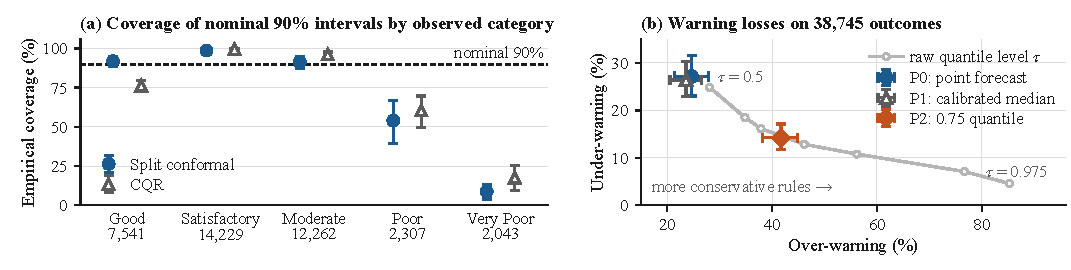
\includegraphics[width=\textwidth]{figures/fig5_uncertainty_warning.pdf}
\caption{RQ3 and RQ4. (a)~Coverage of nominal 90\% intervals by observed category, pooled over 12 folds (95\% intervals; exact pairs under each label). (b)~Conservative rules reduce under-warning and raise over-warning; the grey curve traces raw quantile levels $\tau$.}
\label{fig:uncertainty}
\end{figure*}

\begin{table}[!t]
\caption{Category Warning Losses (\%) on Development Outcomes, Censored Severe Days Included}
\label{tab:warnings}
\centering
\footnotesize
\setlength{\aboverulesep}{0pt}\setlength{\belowrulesep}{0pt}\renewcommand{\arraystretch}{1.14}\setlength{\tabcolsep}{3.6pt}
\begin{tabularx}{\columnwidth}{X r r r r r r}
\toprule
\rowcolor{TableHeader}\textbf{Policy} & \textbf{Folds} & \textbf{$n$} & \textbf{Under} & \textbf{Over} & \textbf{Serious} & \textbf{Poor$+$}\\
\midrule
P0: point forecast & 12 & 38{,}745 & 27.1 & 24.7 & 8.4 & 100.0\\
P1: calibrated median & 12 & 38{,}745 & 26.4 & 23.6 & 7.6 & 100.0\\
P2: 0.75 quantile & 12 & 38{,}745 & 14.2 & 41.7 & 4.1 & 86.3\\
\midrule
P3: 10\% target & 11 & 35{,}306 & 11.1 & 48.7 & 2.8 & 67.8\\
P3: 5\% target & 10 & 32{,}318 & 6.2 & 68.1 & 1.8 & 60.1\\
\bottomrule
\end{tabularx}
\\[3pt]
\parbox{\columnwidth}{\footnotesize Under: issued category below observed. Over: above observed. Serious: at least two bands below. Poor$+$: under-warning among Poor-or-worse outcomes. P3 uses feasible folds only.}
\end{table}


\subsection{RQ4: Warning Trade-Offs}
P0--P2 are scored on the same \nOutcomes{} outcomes (Table~\ref{tab:warnings}). The point rule under-warns on \underPzero\% and over-warns on \overPzero\%; the calibrated median changes little. The 0.75 quantile lowers under-warning by \dUnder{} percentage points (\dUnderLo{} to \dUnderHi{}) and raises over-warning by \dOver{} (\dOverLo{} to \dOverHi{}), a move along an operating curve and not an improvement (Fig.~\ref{fig:uncertainty}b). The curve is steep where it matters: under-warning falls below 5\% only at $\tau = 0.975$, with over-warning on \topOver\% of days. Under-warning among Poor-or-worse outcomes is 100\% for P0 and P1 and \highUnderPtwo\% for P2, and no weather-based rule ever issues Severe. The risk-targeted rule P3 is feasible in \pThreeTenFolds{} and \pThreeFiveFolds{} folds and meets its target in the evaluation month in \pThreeTenMet{} and \pThreeFiveMet{} of them.

\begin{figure*}[!t]
\centering
\setlength{\fboxsep}{0pt}\setlength{\fboxrule}{0.4pt}
\begin{minipage}[t]{0.455\textwidth}\centering
\fcolorbox{PanelRule}{white}{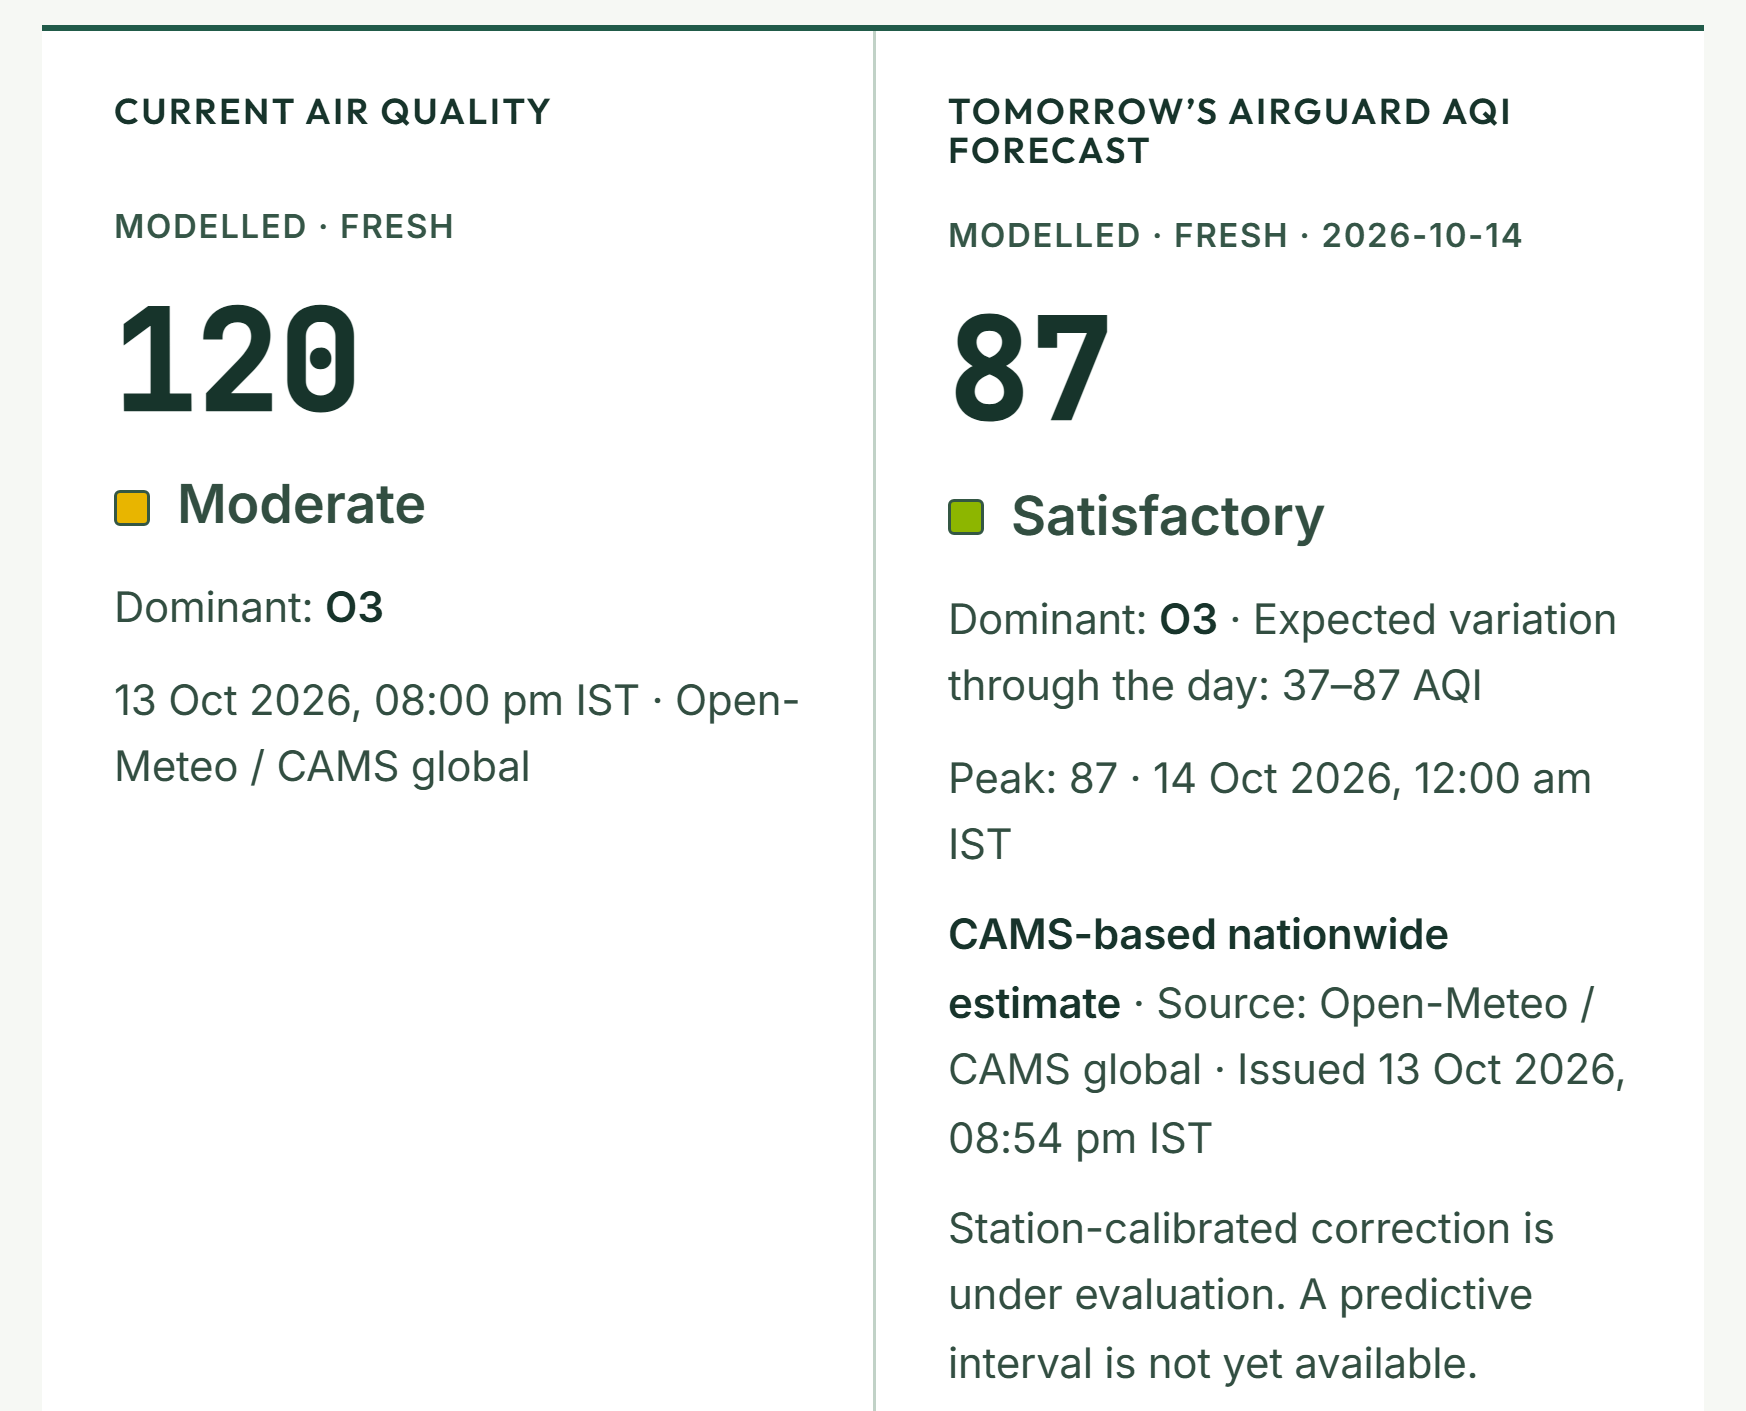
\includegraphics[width=\dimexpr\linewidth-0.8pt\relax]{figures/fig6a_forecast.png}}\\[3pt]
{\footnotesize (a) Operational forecast interface}
\end{minipage}\hspace{0.03\textwidth}%
\begin{minipage}[t]{0.455\textwidth}\centering
\fcolorbox{PanelRule}{white}{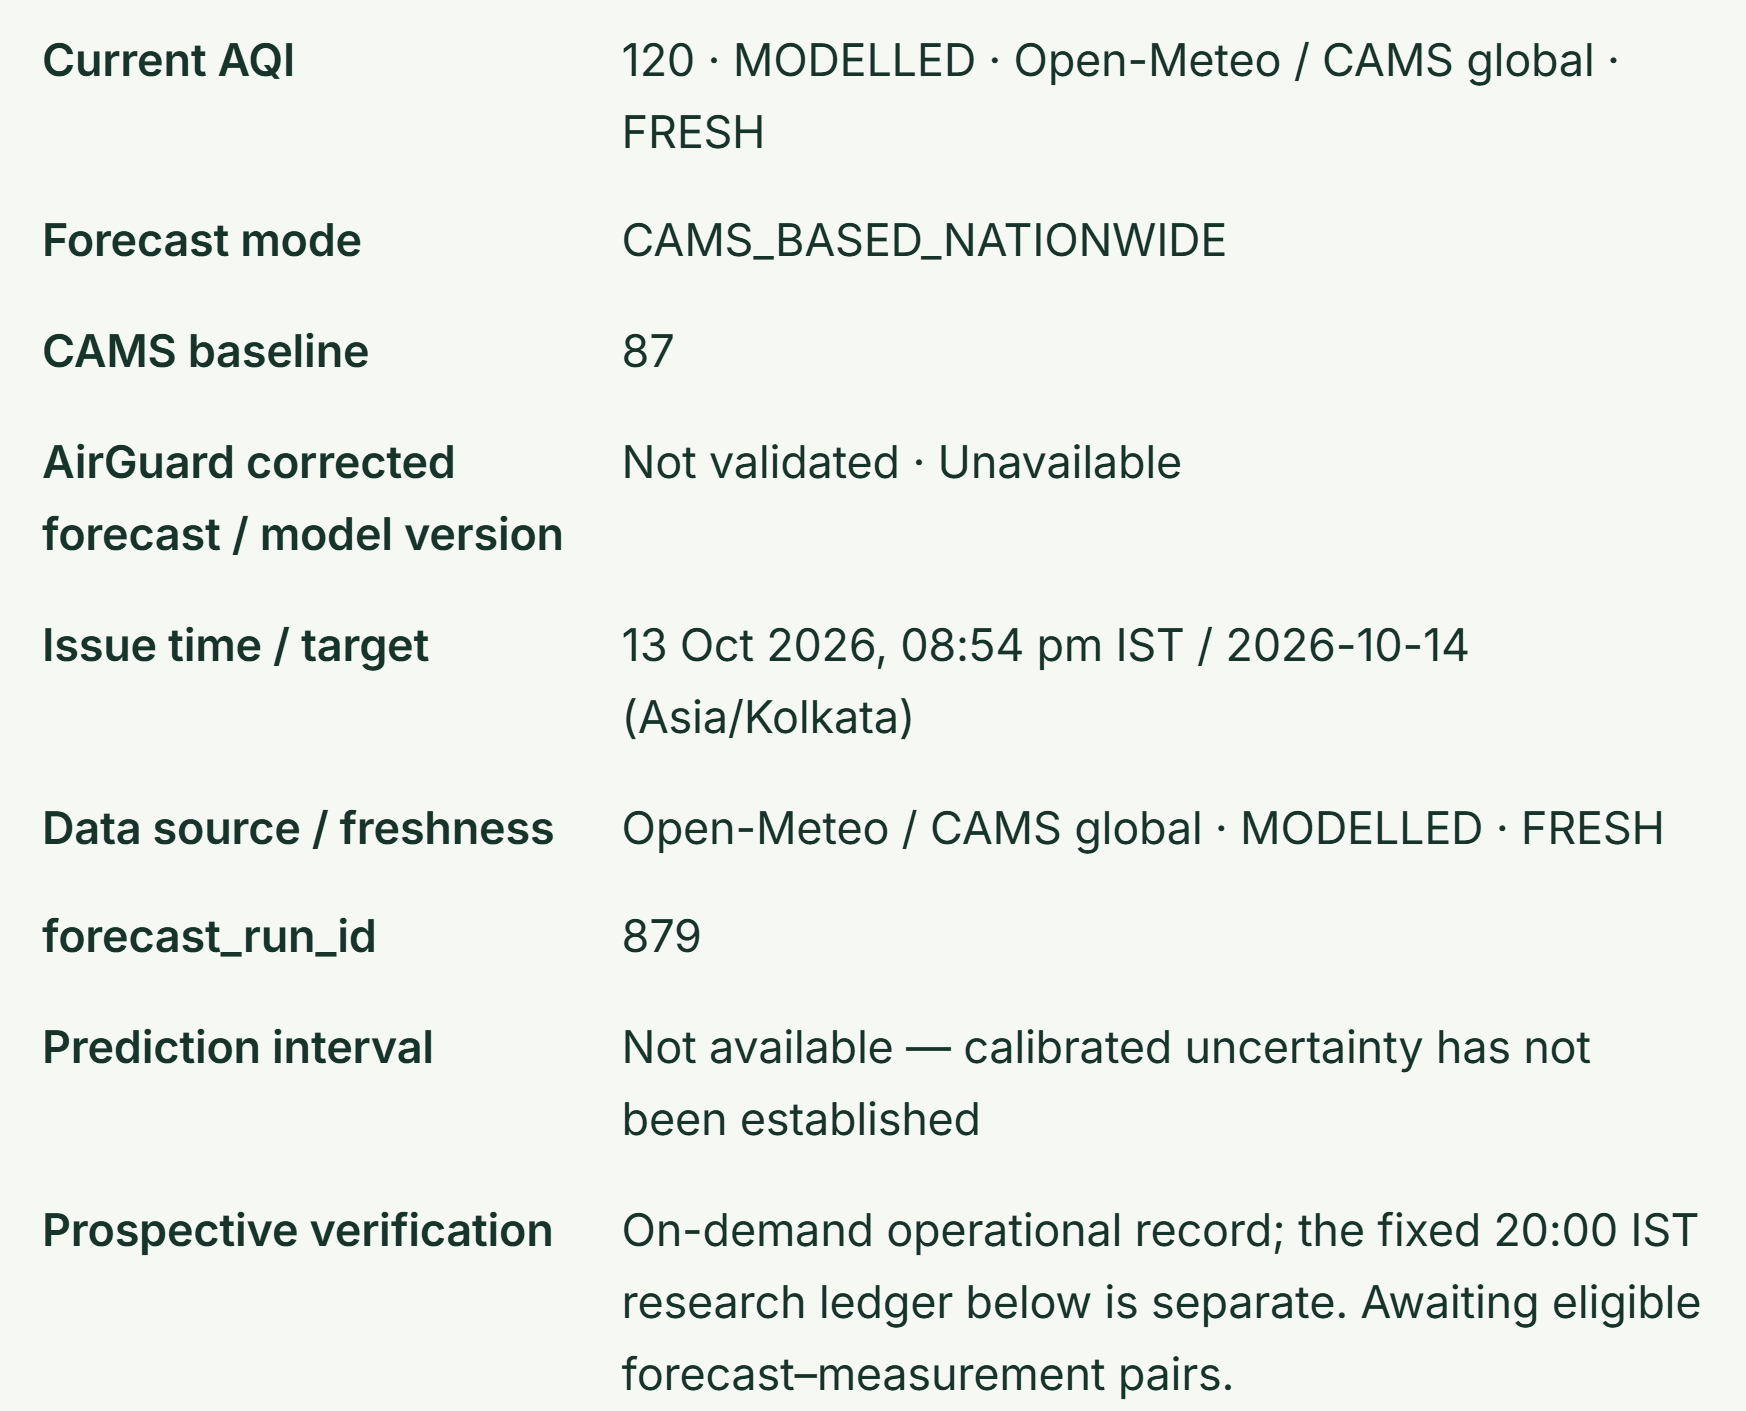
\includegraphics[width=\dimexpr\linewidth-0.8pt\relax]{figures/fig6b_research.png}}\\[3pt]
{\footnotesize (b) Research provenance and validation interface}
\end{minipage}
\caption{Deployed AirGuard India interface (unretouched production captures, 13 October 2026). (a)~Current and next-day AQI with pollutant attribution, source and issue time. (b)~Research status: operational CAMS baseline, correction status, uncertainty availability and prospective verification.}
\label{fig:application}
\end{figure*}

\subsection{Working AirGuard Application}
The availability contract is implemented in a deployed public application (Fig.~\ref{fig:application}) that issues a next-day CPCB-style index for any Indian location through the same AQI engine that builds the research targets. Every value carries a measured or modelled label with its source and issue time, the correction is displayed as not validated, and no predictive interval is offered. The figure demonstrates implementation and provenance transparency, not predictive accuracy: the served estimate is the raw provider product.

\subsection{Insights}
\textit{Mean accuracy can conceal Severe-tail failure.} Weather Ridge lowers average error against climatology, yet its bias reaches \biasWxVeryPoor{} on Very Poor days and it never reaches the Severe lower bound. An average is dominated by days that a warning does not serve.

\textit{Persistence remains a demanding operational baseline.} Episodes last several days, so the index measured before the cutoff already carries most of what a daily linear model can learn; persistence, not climatology, is the reference a future correction must beat~\cite{casciaro2022}.

\textit{Geographic transfer degrades most under pollution.} Withholding a cluster or a region raises pooled error by a few percent but costs several times more on Poor-or-worse days, so national error understates the risk of serving airsheds absent from training~\cite{just2020}.

\textit{Uncertainty and mean accuracy do not determine warning quality.} One monthly residual quantile over-covers clean days while polluted days fall outside, and seasonal onset breaks exchangeability between calibration and evaluation months~\cite{barber2023}. Raising the decision quantile buys fewer missed categories with many more alerts, so under- and over-warning must be evaluated explicitly at a declared operating point. All results are development-stage evidence under the fixed contract, conditional on the assumed three-hour receipt latency.

\section{Conclusion and Future Implementation}
Under an explicit previous-evening availability contract, forecast weather improves the three-pollutant next-day AQI over climatology by \dWxClimAbs{} units and recent measurements add more, yet a history-based Ridge does not establish an advantage over persistence. Geographic exclusion costs little on average and several times more on polluted days. Weather Ridge never reaches the Severe lower bound; among Severe cases with available history, persistence reaches it far more often than the learned history model (\sevPersReach{} against \sevHistReach{} of \nHistSevere{}). Nominal 90\% intervals cover \covNinety\% of exact outcomes but \covSplitVeryPoor\% of Very Poor ones, and conservative warning rules trade missed categories for many more excess alerts. A forecasting system should therefore not be judged by mean error alone: issue-time availability, geographic generalization, behaviour at high severity, severity-conditioned uncertainty and warning costs are separable properties.

Completion of the archived operational CAMS development corpus will enable direct comparison of raw CAMS, climatology, persistence and station-calibrated residual models; the selected configuration will then be frozen in a committed model-selection lock before the protected final interval is evaluated once. A subsequent sensitivity analysis will freeze station eligibility strictly before the development interval to quantify the effect of monitor survivorship on geographic estimates. Severity-aware forecasting will be investigated through quantile and tail-weighted objectives, and uncertainty under changing regimes through adaptive and severity-conditioned conformal recalibration. Pollutant support will extend toward a fuller CPCB index, receipt-time logging will replace the latency assumption, and forecast verification will be surfaced in the deployed interface.

\section*{Acknowledgment}
Generative AI systems (OpenAI ChatGPT and Codex, and Anthropic Claude) drafted manuscript text and analysis and figure code; the author verified all results and references.

\bibliographystyle{IEEEtran}
\bibliography{references}

\end{document}
